% 4_results.tex
\section{Results}
\label{sec:results}

\subsection{Inter-judge agreement is near zero (RQ1)}

Table~\ref{tab:agreement} reports pairwise agreement between the three
judges on the 32 experimental discussions (overall score). No judge
pair reaches substantial rank agreement: $\rho$ spans $-0.05$ to
$+0.47$ (mean $+0.21$), and mean absolute differences run from 0.54 to
0.90 points on a 10-point scale. Per dimension, agreement on insight
depth---the most subjective axis---is near zero or negative for all
three pairs ($-0.23$, $+0.20$, $+0.12$): the judges systematically
disagree about which discussions are deep. All three judges are
distinct models from one vendor, so these figures describe disagreement
across model families within a vendor; whether cross-vendor pairs
disagree more is left to the released artifact as further judges are
added.

\begin{table}[t]
\centering
\caption{Pairwise inter-judge agreement (overall score, 32
discussions).}
\label{tab:agreement}
\small
\begin{tabular}{@{}lccc@{}}
\toprule
Judge pair & $n$ & Spearman $\rho$ & Mean $\lvert\Delta\rvert$ \\
\midrule
step-5-preview vs.\ step-3.7-flash & 32 & $-0.05$ & 0.72 \\
step-5-preview vs.\ step-3.5-flash & 32 & $+0.21$ & 0.90 \\
step-3.7-flash vs.\ step-3.5-flash & 32 & $+0.47$ & 0.54 \\
\bottomrule
\end{tabular}

\smallskip
\noindent Per-dimension $\rho$ on insight depth: $-0.23$, $+0.20$,
$+0.12$ for the three pairs.
\end{table}

\subsection{Leniency offset, not self-preference (RQ2)}

The three judges form a leniency ladder: step-5-preview scores 0.60
above the two-judge mean on a discussion (bootstrap 95\% CI
$[+0.35,+0.84]$, excluding zero), step-3.5-flash scores 0.60 below it
(CI $[-0.81,-0.40]$, excluding zero), and step-3.7-flash sits at the
midpoint ($+0.01$, CI $[-0.18,+0.21]$). The two extreme judges thus
differ by roughly 1.2 points on the 10-point scale for identical
transcripts. Crucially, the offsets persist in cells where the judge
did \emph{not} produce the discussion, so they are properties of the
judges, not preferences for their own family. Direct self-preference
estimates are small and statistically indistinguishable from zero:
$+0.05$ (CI $[-0.70,+0.70]$) and $-0.10$ (CI $[-0.40,+0.40]$) for the
two judges that also served as drivers. This decomposes the two
mechanisms that the standard mitigation (``use a different family'')
conflates: changing family removes self-preference, which was not the
operative effect here, while leaving the leniency offset untouched.

\begin{table}[t]
\centering
\caption{Leniency offset per judge (score minus the mean of the other
judges on the same discussion) and self-preference delta (same-driver
minus other-driver discussions), with bootstrap 95\% intervals
(10{,}000 resamples).}
\label{tab:leniency}
\small
\begin{tabular}{@{}lccc@{}}
\toprule
Judge & Leniency offset & 95\% CI & Self-pref.\ $\Delta$ (CI) \\
\midrule
step-5-preview & $+0.60$ & $[+0.35,+0.84]$ & $+0.05$ ($[-0.70,+0.70]$) \\
step-3.7-flash & $+0.01$ & $[-0.18,+0.21]$ & $-0.10$ ($[-0.40,+0.40]$) \\
step-3.5-flash & $-0.60$ & $[-0.81,-0.40]$ & --- \\
\bottomrule
\end{tabular}
\end{table}

\subsection{Single-judge component conclusions do not replicate (RQ3)}

Table~\ref{tab:ablation} reports the ablation replication at five
repetitions per condition under the primary driver. Judge A ranks the
full system \emph{below} both ablations (Cliff's $\delta=-0.48$ and
$-0.64$): removing components \emph{raises} the score. Judges B and C
run in the opposite direction, consistent with the audited evaluation's
ordering but with small effect sizes. The audited evaluation's headline
claim---that arbitration and jitter contribute $-0.92$ and $-0.80$---is
reproduced by \emph{no} judge at anything like that magnitude.

\begin{table}[t]
\centering
\caption{Ablation replication, five repetitions per condition, primary
driver (mean overall $\pm$ SD). $\delta$ is Cliff's delta for full
vs.\ ablated condition under the stated judge.}
\label{tab:ablation}
\small
\begin{tabular}{@{}lcccccc@{}}
\toprule
& \multicolumn{2}{c}{Judge A} & \multicolumn{2}{c}{Judge B} & \multicolumn{2}{c}{Judge C} \\
\cmidrule(lr){2-3}\cmidrule(lr){4-5}\cmidrule(lr){6-7}
Condition & Score & $\delta$ & Score & $\delta$ & Score & $\delta$ \\
\midrule
Full system & $6.56\pm.57$ & --- & $6.24\pm.26$ & --- & $5.84\pm.70$ & --- \\
No arb.\ (round-robin) & $7.04\pm.41$ & $-0.48$ & $6.04\pm.17$ & $+0.56$ & $5.76\pm.57$ & $+0.16$ \\
No jitter & $7.12\pm.30$ & $-0.64$ & $6.04\pm.74$ & $+0.08$ & $5.52\pm.93$ & $+0.28$ \\
\bottomrule
\end{tabular}
\end{table}

\subsection{Same-machine replication: only the judge varies}

Table~\ref{tab:samemachine} holds transcripts fixed and varies only the
judge, on the secondary driver (three repetitions per condition). A
same-model judge---the structure of the audited single-judge
protocol---ranks the full system \emph{below} the no-jitter ablation
($\delta=-0.56$); cross-model judge A ranks it below the round-robin
ablation at the maximum effect size ($\delta=-1.00$: every round-robin
discussion outscores every full-system discussion); cross-model judge B
places it first on both comparisons but with small effects. Across both
drivers and all three judges, no judge--driver combination reproduces
the audited evaluation's component ordering: the ranking is a property
of the judge, not of the system.

\begin{table}[t]
\centering
\caption{Same-machine replication (secondary driver, three repetitions
per condition, mean overall $\pm$ SD). Identical transcripts; only the
judge differs.}
\label{tab:samemachine}
\small
\begin{tabular}{@{}lcccccc@{}}
\toprule
& \multicolumn{2}{c}{Same-model} & \multicolumn{2}{c}{Cross-model A} & \multicolumn{2}{c}{Cross-model B} \\
\cmidrule(lr){2-3}\cmidrule(lr){4-5}\cmidrule(lr){6-7}
Condition & Score & $\delta$ & Score & $\delta$ & Score & $\delta$ \\
\midrule
Full system & $6.27\pm.58$ & --- & $6.13\pm.12$ & --- & $6.40\pm.72$ & --- \\
No arb.\ (round-robin) & $6.47\pm.12$ & $+0.11$ & $6.80\pm.35$ & $-1.00$ & $6.13\pm.12$ & $+0.33$ \\
No jitter & $6.93\pm.64$ & $-0.56$ & $5.93\pm1.03$ & $-0.11$ & $5.93\pm.83$ & $+0.33$ \\
\bottomrule
\end{tabular}
\end{table}

\subsection{Mechanism metrics: the framework operates as designed}
\label{sec:mechanism}

Judge-free metrics confirm the ablations manipulate what they claim.
Under the primary driver, the full system produces unequal speaking
counts (Gini $=0.10$), round-robin produces a fixed rotation (Gini
$=0.00$ at three rounds; $0.13$ at five), and removing jitter collapses
most of the asymmetry (Gini $=0.03$), confirming jitter as the
operative source of speaking inequality. Forced speech never occurs
under round-robin (by construction) and occurs under both other
conditions. The framework's speaking mechanism behaves as documented;
the instability documented above resides in the evaluation layer, not
the framework.

\begin{table}[t]
\centering
\caption{Mechanism metrics per ablation condition (deterministic, no
judge involved). Gini: speaking-count inequality; forced: rounds in
which all agents waited and a speaker was forced.}
\label{tab:mechanism}
\small
\begin{tabular}{@{}lcccc@{}}
\toprule
& \multicolumn{2}{c}{Primary driver} & \multicolumn{2}{c}{Secondary driver} \\
\cmidrule(lr){2-3}\cmidrule(lr){4-5}
Condition & Gini & Forced & Gini & Forced \\
\midrule
Full system & 0.10 & 5/25 & 0.23 & 1/9 \\
No arbitration & 0.00--0.13 & 0/25 & 0.13 & 0/9 \\
No jitter & 0.03 & 5/25 & 0.19 & 1/9 \\
\bottomrule
\end{tabular}
\end{table}

\begin{figure}[t]
\centering
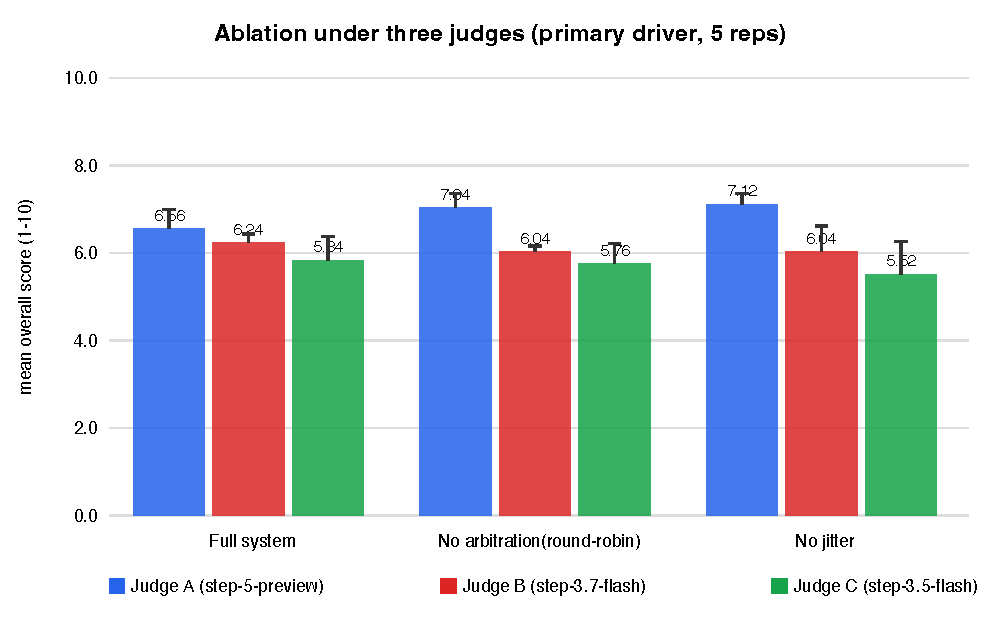
\includegraphics[width=0.85\linewidth]{figures/fig1_condition_scores}
\caption{Per-condition scores under three judges with bootstrap
intervals (primary driver, five repetitions). The ordering of
conditions varies across judges.}
\label{fig:flip}
\end{figure}

\begin{figure}[t]
\centering
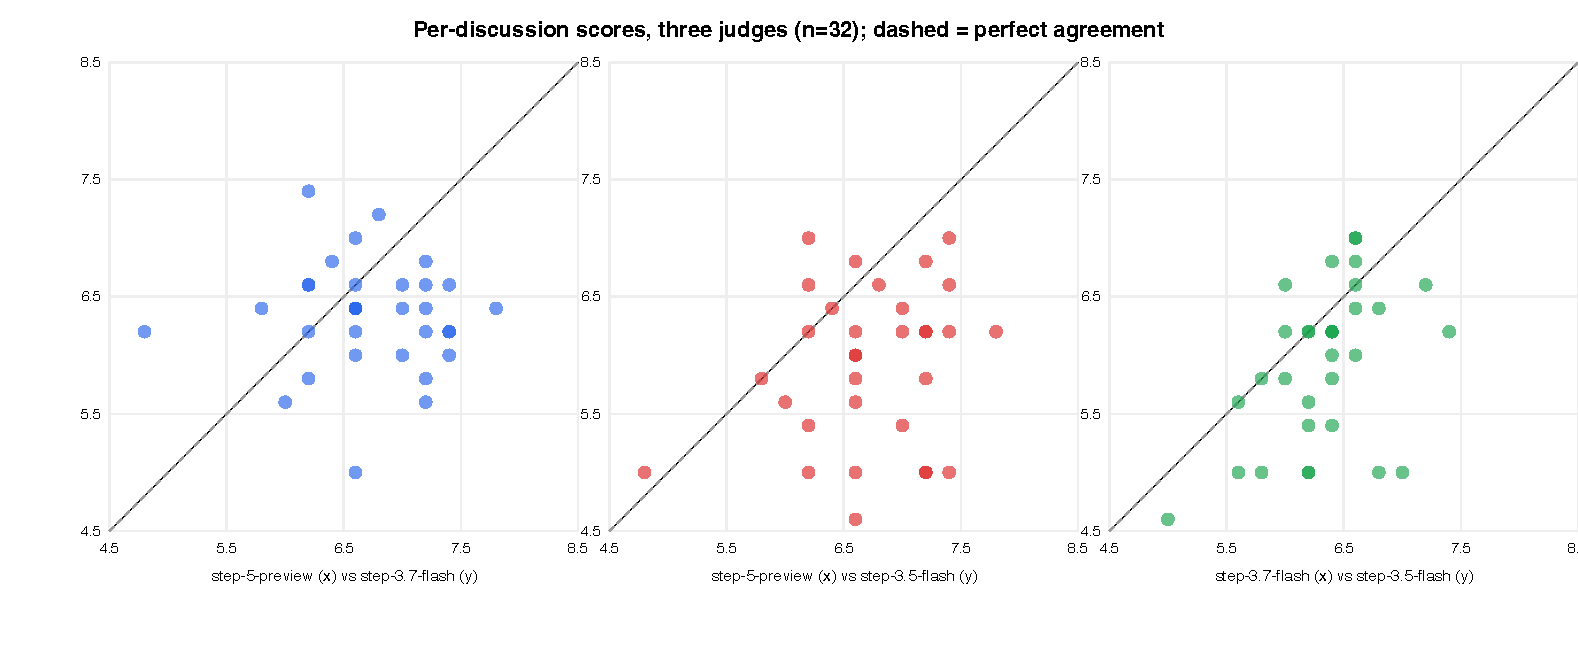
\includegraphics[width=0.85\linewidth]{figures/fig2_trajectories}
\caption{Per-discussion overall scores for all three judge pairs
(32 discussions). No pair shows tight agreement.}
\label{fig:trajectories}
\end{figure}

\begin{figure}[t]
\centering
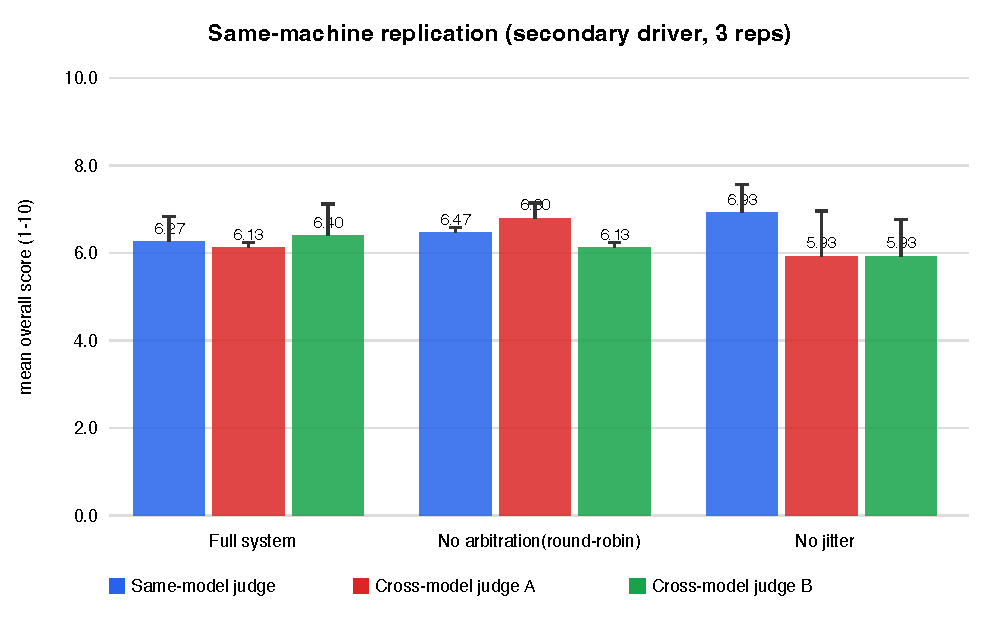
\includegraphics[width=0.85\linewidth]{figures/fig3_same_machine}
\caption{Same-machine replication: identical transcripts scored by three
judges (secondary driver). The full system leads under at most one
judge.}
\label{fig:samemachine}
\end{figure}

\begin{figure}[t]
\centering
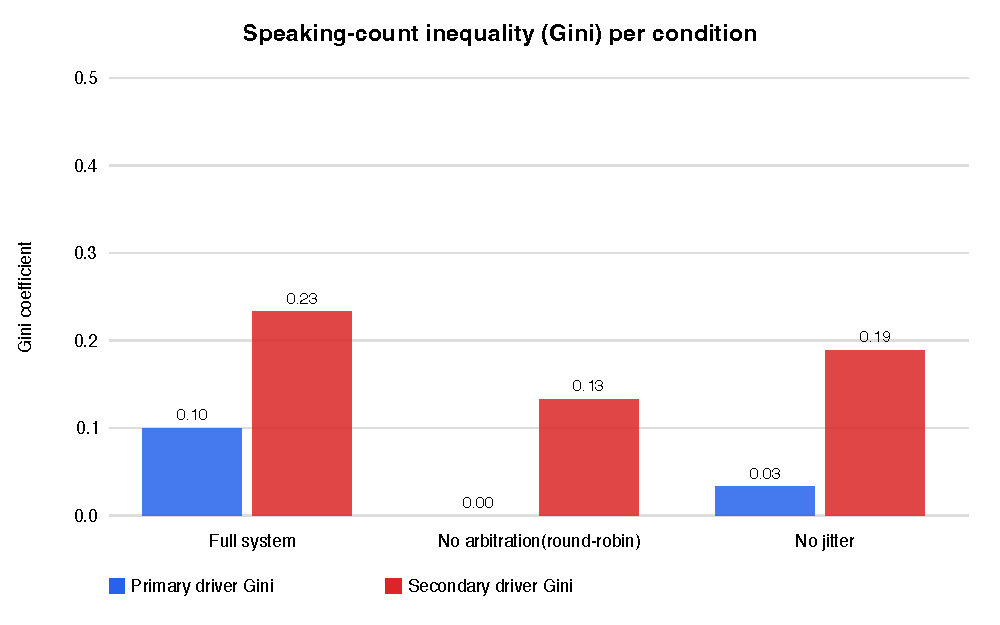
\includegraphics[width=0.85\linewidth]{figures/fig4_mechanism}
\caption{Mechanism metrics per condition (speaking Gini and forced
rounds), both drivers. Jitter removal collapses speaking asymmetry
under the primary driver.}
\label{fig:mechanism}
\end{figure}
